\section{Experiments}
\label{sec:experiments}

\subsection{Protocol}

\textbf{Baseline.} HybridGL \cite{liu2025hybridgl} at its own released
operating point, re-implemented from the official code. We report both the
\emph{unguided} row (argmax of the semantic score over the full pool, i.e.\ the
``G2L alone'' configuration of the paper's ablation) and the \emph{released
guidance} row (Eq.~\ref{eq:released}).

\textbf{Proposer and scorer.} SAM ViT-H with
\texttt{points\_per\_side}\,$=8$, \texttt{pred\_iou\_thresh}\,$=0.7$,
\texttt{stability\_score\_thresh}\,$=0.7$, \texttt{min\_mask\_region\_area}\,$=800$,
\texttt{crop\_n\_layers}\,$=0$, giving 48.4 proposals per image on average; CLIP
ViT-B/16 with HybridGL's G2L fusion, \texttt{masking\_block}\,$=9$. All features
are computed once and cached; every result below is a re-analysis of one stored
pass.

\textbf{Data.} Full validation splits: RefCOCO val (10{,}834 expressions,
1{,}500 images), RefCOCO$+$ val (10{,}758), RefCOCOg val / UMD (4{,}896).

\textbf{Metrics.} mIoU (per-expression mean, primary) and oIoU (dataset-level).
\textbf{Oracle mIoU} is reported for every pool because it is the
scorer-independent reference point.

\textbf{Statistics.} Every reported delta is paired over expressions with a
10{,}000-resample bootstrap (95\,\% CI) and a sign-flip permutation test
($p$), with win/loss counts. Any hyper-parameter is selected on a
716-expression split of RefCOCO val (250 references, fixed seed, chosen before
the final script was written) and reported on the full split and on the
held-out complement.

\subsection{Reproduction}

On RefCOCO val our reproduction reaches 0.3518 mIoU / 0.2768 oIoU unguided and
0.4482 / 0.3816 with the released guidance, against the published 40.27 / 31.71
and 49.48 / 41.81. The absolute shortfall is real and §\ref{sec:repro}
localises it. We report it because it bounds the reading of every absolute
number: all comparisons in this paper are internal to one reproduction, and
absolute rows are not directly comparable to the published table.

\subsection{Main result}

\begin{table*}[t]
\caption{Full RefCOCO validation split, 10{,}834 expressions, released HybridGL
scorer. Oracle mIoU 0.8221. $\dD$ is paired over expressions; CI is a
10{,}000-resample bootstrap; $p$ is a sign-flip permutation test; every
$p<0.0001$. ``changed'' counts expressions whose returned index differs from the
released row. All deltas are computed from unrounded values, so a delta may
differ by $\pm 0.0001$ from the difference of the two rounded mIoU columns
shown. The containment snap is a required baseline and is \emph{not} part of
the proposed method.}
\label{tab:main}
\centering
\small
\begin{tabular}{lccccccc}
\toprule
row & mIoU & oIoU & $\dD$ vs released [95\,\% CI] & $\dD$ vs argmax & changed & win & loss \\
\midrule
HybridGL argmax (unguided)      & 0.3518 & 0.2768 & $-0.0964\,[-0.1030,-0.0898]$ & ---     & 4746 & 1005 & 2840 \\
HybridGL released guidance      & 0.4482 & 0.3816 & ---                            & $+0.0964$ & 0    & ---  & ---  \\
\;+ containment snap (baseline) & 0.5024 & 0.4072 & $+0.0541\,[+0.0505,+0.0578]$ & $+0.1505$ & 2995 & 1826 & 421  \\
\;\textbf{+ ours}               & \best{0.5029} & \best{0.4431} & \best{$+0.0546\,[+0.0493,+0.0601]$} & \best{$+0.1510$} & 2865 & 1721 & 764 \\
\;+ ours + snap (composition)   & 0.5505 & 0.4574 & $+0.1023\,[+0.0963,+0.1083]$ & $+0.1987$ & 4284 & 2850 & 826 \\
\bottomrule
\end{tabular}
\end{table*}

\begin{table}[t]
\caption{Sensitivity of the operator on full RefCOCO val. The shipped
configuration ($k=8$, side percentile 50, category score, coherence ranking) was
fixed on the 716-expression selection split before the final evaluation script
and is not the best cell of any sweep.}
\label{tab:sensitivity}
\centering
\footnotesize
\setlength{\tabcolsep}{4pt}
\begin{tabular}{@{}lccl@{}}
\toprule
variant & mIoU & oIoU & $\dD$ vs released \\
\midrule
shipped ($k=8$)          & \best{0.5029} & \best{0.4431} & \best{$+0.0546$} \\
$k=5$                    & 0.4880 & 0.4241 & $+0.0397$ \\
$k=12$                   & 0.5050 & 0.4474 & $+0.0568$ \\
$k=16$                   & 0.5038 & 0.4470 & $+0.0555$ \\
$k=24$                   & 0.5018 & 0.4453 & $+0.0535$ \\
side percentile 34       & 0.4938 & 0.4378 & $+0.0455$ \\
side percentile 66       & 0.5016 & 0.4389 & $+0.0534$ \\
set: stripped text        & 0.4999 & 0.4377 & $+0.0517$ \\
set: full expression      & 0.4938 & 0.4317 & $+0.0455$ \\
set: noun probe           & 0.4919 & 0.4334 & $+0.0437$ \\
\bottomrule
\end{tabular}
\end{table}

Table~\ref{tab:main} gives the main result. The operator raises the released
pipeline on full RefCOCO val from 0.4482 to 0.5029 mIoU and from 0.3816 to
0.4431 oIoU; the delta is $+0.0546$ mIoU (95\,\% CI $[+0.0493,+0.0601]$,
$p<0.0001$) with 1{,}721 expressions improved and 764 degraded. Against the
unguided argmax the gain is $+0.1510$ mIoU. The oracle-hit rate --- the fraction
of expressions whose returned proposal is exactly the best pool member --- rises
from 0.454 to 0.516. Table~\ref{tab:sensitivity} shows the operator is not
tuned to a peak: $k\in\{5,12,16,24\}$ gives $+0.0397$ to $+0.0568$, the
side-split percentile gives $+0.0455$ to $+0.0546$, and the set source gives
$+0.0437$ to $+0.0546$. On the held-out complement of the selection split
($n=10{,}118$) the delta is $+0.0540\,[+0.0482,+0.0599]$.

\subsection{The operator and the containment snap are complementary, not
competing}
\label{sec:snap}

The most demanding baseline here is a one-line containment snap: replace the
selected mask by the smallest pool proposal that covers at least 95\,\% of it.
It is the operator that previously explained away an earlier method of ours,
and it is included as a required row.

On mIoU the two are \emph{statistically indistinguishable}: a paired bootstrap
on the per-expression difference of the two deltas gives
$+0.0005\,[-0.0055,+0.0066]$, $p=0.87$. We state this plainly rather than
reporting the point estimate that favours us. They act on largely different
expressions, however --- ours is strictly better on 1{,}324, the snap on
1{,}323, with 7{,}314 ties; ours gains where the snap hurts on 45 expressions
and the snap gains where ours hurts on 119 --- and they separate on everything
else that matters:

\begin{itemize}
\item \textbf{oIoU: 0.4431 vs 0.4072} ($+3.6$ points). The selector moves the
dataset-level metric; the snap moves mIoU only.
\item \textbf{Part expressions} ($n=443$): $+0.0439$ versus $+0.0345$.
\item \textbf{GT-area quartiles}: ours is positive in all four
($+0.0329 / +0.0500 / +0.0561 / +0.0795$); the snap's gain is confined to the
largest quartile by construction, and it is $+0.0136$ on part expressions at
the unguided point.
\end{itemize}

Because the two fix different error classes --- wrong-instance and
under-segmentation, §\ref{sec:diagnosis} --- they compose almost additively:
applying the snap after the selector gives $0.5505$ mIoU / $0.4574$ oIoU, i.e.\
$+0.1023$ over the released pipeline. We attribute that row explicitly to the
composition rather than to the selector.

\subsection{Controls}
\label{sec:controls}

\begin{table}[t]
\caption{Controls on full RefCOCO val. Each replaces one component of the
operator and leaves the rest intact.}
\label{tab:controls}
\centering
\footnotesize
\setlength{\tabcolsep}{4pt}
\begin{tabular}{@{}lcl@{}}
\toprule
control & $\dD$ mIoU & reading \\
\midrule
geometric extremum of the set & $-0.0549$ & not ``take the leftmost'' \\
rank by category score        & $-0.0024$ & semantic re-ranking is inert \\
rank by full semantic score   & $-0.0117$ & idem \\
mirror the relation           & $-0.1813$ & the relation semantics are real \\
whole pool instead of top-8   & $+0.0484$ & category set: $+0.006$ \\
coherence ranking, no gate    & $+0.0430$ & side gate: $+0.012$ \\
\bottomrule
\end{tabular}
\end{table}

Table~\ref{tab:controls} isolates the mechanism. Picking the geometric extremum
of the candidate set instead of ranking by coherence is \emph{worse than doing
nothing} ($-0.0549$): the operator is not a heuristic preference for extreme
positions. Ranking by the semantic score instead of the released coherence
score gives $-0.0024$ (category score) and $-0.0117$ (full score): the semantic
score cannot choose within the set, which is exactly the failure the diagnosis
describes. Mirroring the relation --- the text says \emph{left}, the resolver
takes the rightmost --- costs $-0.1813$, confirming that the relation's
semantics rather than any extreme pick carry the gain. Finally, running the
same ranking over the whole pool rather than the top-8 category set gives
$+0.0484$, and dropping the relation gate gives $+0.0430$.

The decomposition, stated plainly: of the $+0.0546$ total, roughly $+0.043$
comes from allowing the released coherence and position machinery to act on
more than its top-3 candidates, $+0.012$ from gating on the parsed relation,
and $+0.006$ from building the set with the category score rather than the full
expression. The first term is the largest, and it is a structural property of
the baseline, not a component we designed.

\subsection{Stratification}

By relation type: horizontal ($n=4{,}749$) $+0.1076$; vertical ($n=443$)
$+0.0735$; middle ($n=584$) $+0.0820$; ordinal ($n=444$) $0.0000$ (abstains,
§\ref{sec:method}); no relation ($n=4{,}614$) $0.0000$ by construction. The
operator never touches an expression it cannot parse, so the 42.6\,\% of
expressions without a spatial relation are bit-identical to the baseline.

By GT-area quartile the gain is positive throughout
($+0.0329 / +0.0500 / +0.0561 / +0.0795$), in contrast to the containment snap
whose benefit is concentrated in large objects. Part expressions gain
$+0.0439$.

\subsection{Candidate-set ceilings}

For any chooser --- including a multimodal model --- acting on a given
candidate set, the best achievable mIoU is the mean over expressions of the
best pool member inside that set. On full RefCOCO val: the released top-3 set
admits $0.5812$ (the released pipeline achieves $0.4482$, i.e.\ 61\,\% of it);
the operator's top-8 category set admits $0.7303$ (the operator achieves
$0.5029$, 47\,\% of it); the whole pool admits $0.8221$. The operator's
candidate set therefore raises the ceiling by $+0.149$ mIoU and captures
roughly half of it, and at most $+0.227$ mIoU remains available to a better
chooser operating on the same set. This bound is the frame in which the absence
of a multimodal chooser baseline should be read (§\ref{sec:limitations}).

\subsection{Reproduction gap, localised}
\label{sec:repro}

The published ablation of HybridGL gives G2L alone $31.71$ oIoU / $40.27$ mIoU
and G2L with all three guidance modules $41.81$ / $49.48$ on RefCOCO val, i.e.\
a guidance increment of $+10.10$ oIoU / $+9.21$ mIoU. Our reproduction's
guidance increment is $+10.48$ / $+9.64$ --- within 0.4 points. The entire
shortfall therefore lies in the frozen feature/score path, not in the guidance
we re-implemented:

\begin{center}
\footnotesize
\begin{tabular}{lcc}
\toprule
dataset & base (G2L) gap & guidance gap \\
\midrule
RefCOCO val  & $-4.03$ oIoU / $-5.09$ mIoU & $+0.38$ / $+0.43$ \\
RefCOCOg val & $-2.32$ / $-2.16$            & $+1.29$ / $+0.99$ \\
\bottomrule
\end{tabular}
\end{center}

This matters twice over. It establishes that the guidance modules --- the
component our operator interacts with --- are faithfully reproduced, and it
scopes the absolute numbers: a better base feature path would raise both rows
together and is orthogonal to this paper's claim.

\subsection{Pool density does not explain the diagnosis}

\begin{table}[t]
\caption{Proposal-pool density on the identical 716 selection-split
expressions. Doubling the pool buys $+1.0$ mIoU of oracle while degrading the
released pipeline by $3.2$ mIoU, and leaves both the diagnosis and the operator
intact.}
\label{tab:pool}
\centering
\small
\begin{tabular}{lccc}
\toprule
& \texttt{pps}$=8$ & \texttt{pps}$=16$ \\
\midrule
proposals / image        & 48.4 & 101.7 \\
oracle mIoU              & 0.8285 & 0.8388 \\
released mIoU            & 0.4700 & 0.4383 \\
wrong-instance gap share & 0.741 & 0.720 \\
\;\;prevalence            & 0.344 & 0.363 \\
under-segmentation share & 0.205 & 0.226 \\
ours mIoU                & 0.5329 & 0.4968 \\
$\dD$ vs released        & $+0.0629$ & $+0.0585$ \\
$\dD$ on spatial stratum & $+0.1041$ & $+0.0968$ \\
\bottomrule
\end{tabular}
\end{table}

Every other measurement in this paper uses one pool. If the diagnosis were an
artefact of a sparse pool, a denser one would dissolve it. Table~\ref{tab:pool}
re-runs the entire released pipeline with SAM at \texttt{points\_per\_side}
$=16$ on the identical 716 expressions ($+110\,\%$ proposals, 48.4
$\rightarrow$ 101.7 per image).

Doubling the pool buys only $+1.0$ mIoU of oracle, which is the diagnosis in
one number: the pool was not the constraint. Worse for the pool-centric view,
the released pipeline \emph{degrades} by $3.2$ mIoU, because a denser pool adds
distractors and the selector must now choose among more of them. The
wrong-instance share of the gap is stable ($0.741 \rightarrow 0.720$), and the
operator still works ($+0.0629 \rightarrow +0.0585$ overall, $+0.1041
\rightarrow +0.0968$ on spatial expressions). A better pool does not repair
selection failure; it concentrates it.

\subsection{Cross-dataset behaviour, and the boundary of the repair}
\label{sec:cross}

\begin{table*}[t]
\caption{Cross-dataset behaviour of the operator at the released HybridGL
operating point. The three splits differ sharply, and for construction reasons,
in how often an expression carries a spatial relation: RefCOCO$+$ was collected
with location words excluded. ``$\dD$ fired'' is the delta restricted to
expressions whose returned index the operator changed. Wrong-instance share is
the fraction of the oracle gap mass that class carries.}
\label{tab:cross}
\centering
\small
\begin{tabular}{lccccccccc}
\toprule
dataset & $n$ & spatial\,\% & fires\,\% & released mIoU & ours mIoU & $\dD$ all & $\dD$ spatial & $\dD$ fired & wrong-inst.\ share \\
\midrule
RefCOCO   & 10{,}834 & 57.4 & 26.4 & 0.4482 & 0.5029 & \best{$+0.0546$} & $+0.0951$ & $+0.2065$ & 0.774 \\
RefCOCOg  & 4{,}896  & 17.7 & 8.3  & 0.5008 & 0.4974 & $-0.0034$ & $-0.0191$ & $-0.0406$ & 0.864 \\
RefCOCO$+$ & 10{,}758 & \best{1.6} & 0.8 & 0.4023 & 0.4035 & $+0.0012$ & $+0.0791$ & $+0.1591$ & 0.801 \\
\bottomrule
\end{tabular}
\end{table*}

\begin{figure}[t]
\centering
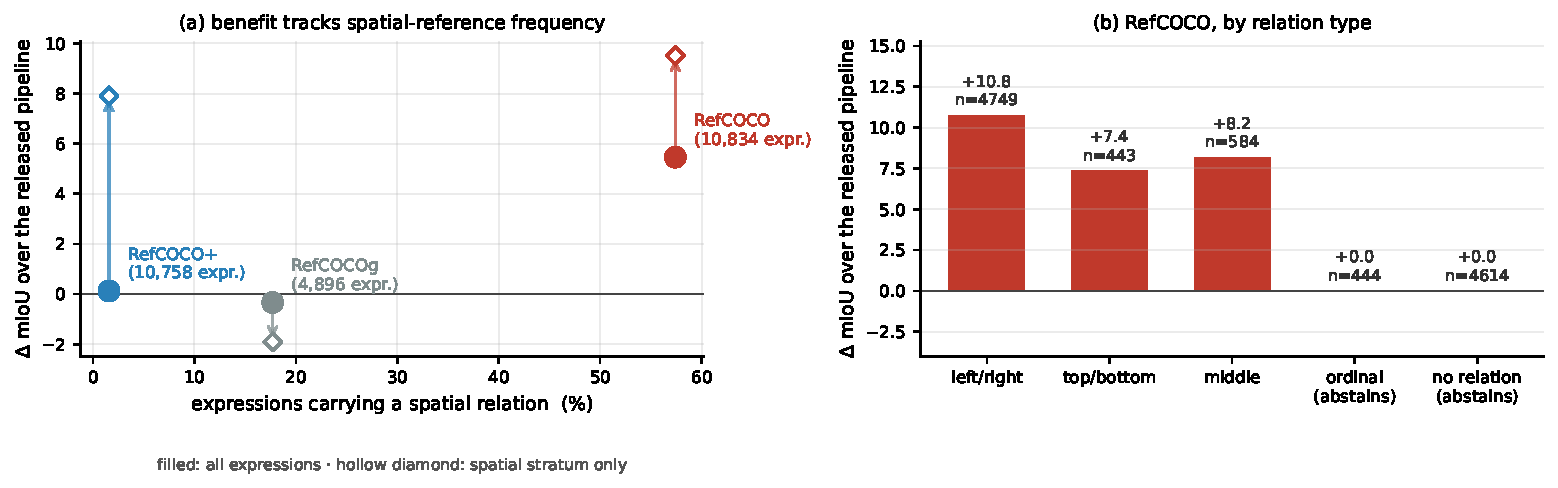
\includegraphics[width=\columnwidth]{figures/dose_response.pdf}
\caption{(a) The operator's benefit tracks how often expressions carry a
spatial relation. Filled markers: all expressions; hollow diamonds: the spatial
stratum only. The RefCOCO$+$ outcome was predicted before the run, from the
dataset's construction. (b) Deltas by relation type on RefCOCO. Ordinal and
relation-free expressions are unchanged by construction.}
\label{fig:dose}
\end{figure}

Table~\ref{tab:cross} and Fig.~\ref{fig:dose} report the operator on all three
splits. Three readings.

\textbf{The diagnosis transfers.} Wrong-instance carries 77.4\,\%, 86.4\,\% and
80.1\,\% of the recoverable IoU on RefCOCO, RefCOCOg and RefCOCO$+$
respectively, all at the released operating point; on RefCOCO it carries
82.2\,\% at the unguided point as well, and 72.0--74.1\,\% at both pool
densities tested. The central claim therefore holds on all three standard
benchmarks, at two operating points on RefCOCO, and at two pool densities.

\textbf{The repair does not transfer uniformly, and the reason is
measurable.} RefCOCO$+$ contains a spatial word in only 1.6\,\% of its
expressions, by construction; the operator fires on 0.8\,\% of them and is
neutral overall ($+0.0012$). RefCOCOg occupies the middle (17.7\,\%) and is
also neutral ($-0.0034$). RefCOCO, at 57.4\,\%, gains $+0.0546$.

\textbf{The neutral RefCOCO$+$ result is a low-information null, not a
failure, and we test it that way.} A neutral overall number would be
uninformative if the operator were simply broken there. Restricted to the
1.6\,\% of RefCOCO$+$ expressions that do carry a spatial relation, the
operator gains $+0.0791$ overall, with $+0.0558$ / $+0.0944$ / $+0.1311$ on the
horizontal ($n=8$) / vertical ($n=105$) / middle ($n=23$) sub-strata. The two
substantive sub-strata have the same sign and comparable magnitude as on
RefCOCO. The horizontal sub-stratum has $n=8$ and we do not draw conclusions
from it.

RefCOCOg is the genuine exception: neutral overall \emph{and} slightly negative
on its own spatial stratum (horizontal $+0.0149$, $n=563$; vertical $-0.1266$,
$n=176$; middle $-0.0342$, $n=78$). RefCOCOg's expressions are long and
predominantly \emph{object-relative} (``the man on the left in the blue shirt'',
``the bird above the branch''), for which an image-frame coordinate resolver is
the wrong instrument. We report this as a boundary with a hypothesis rather
than tuning the operator until the hypothesis fits.

\subsection{Qualitative behaviour}

\begin{figure*}[t]
\centering
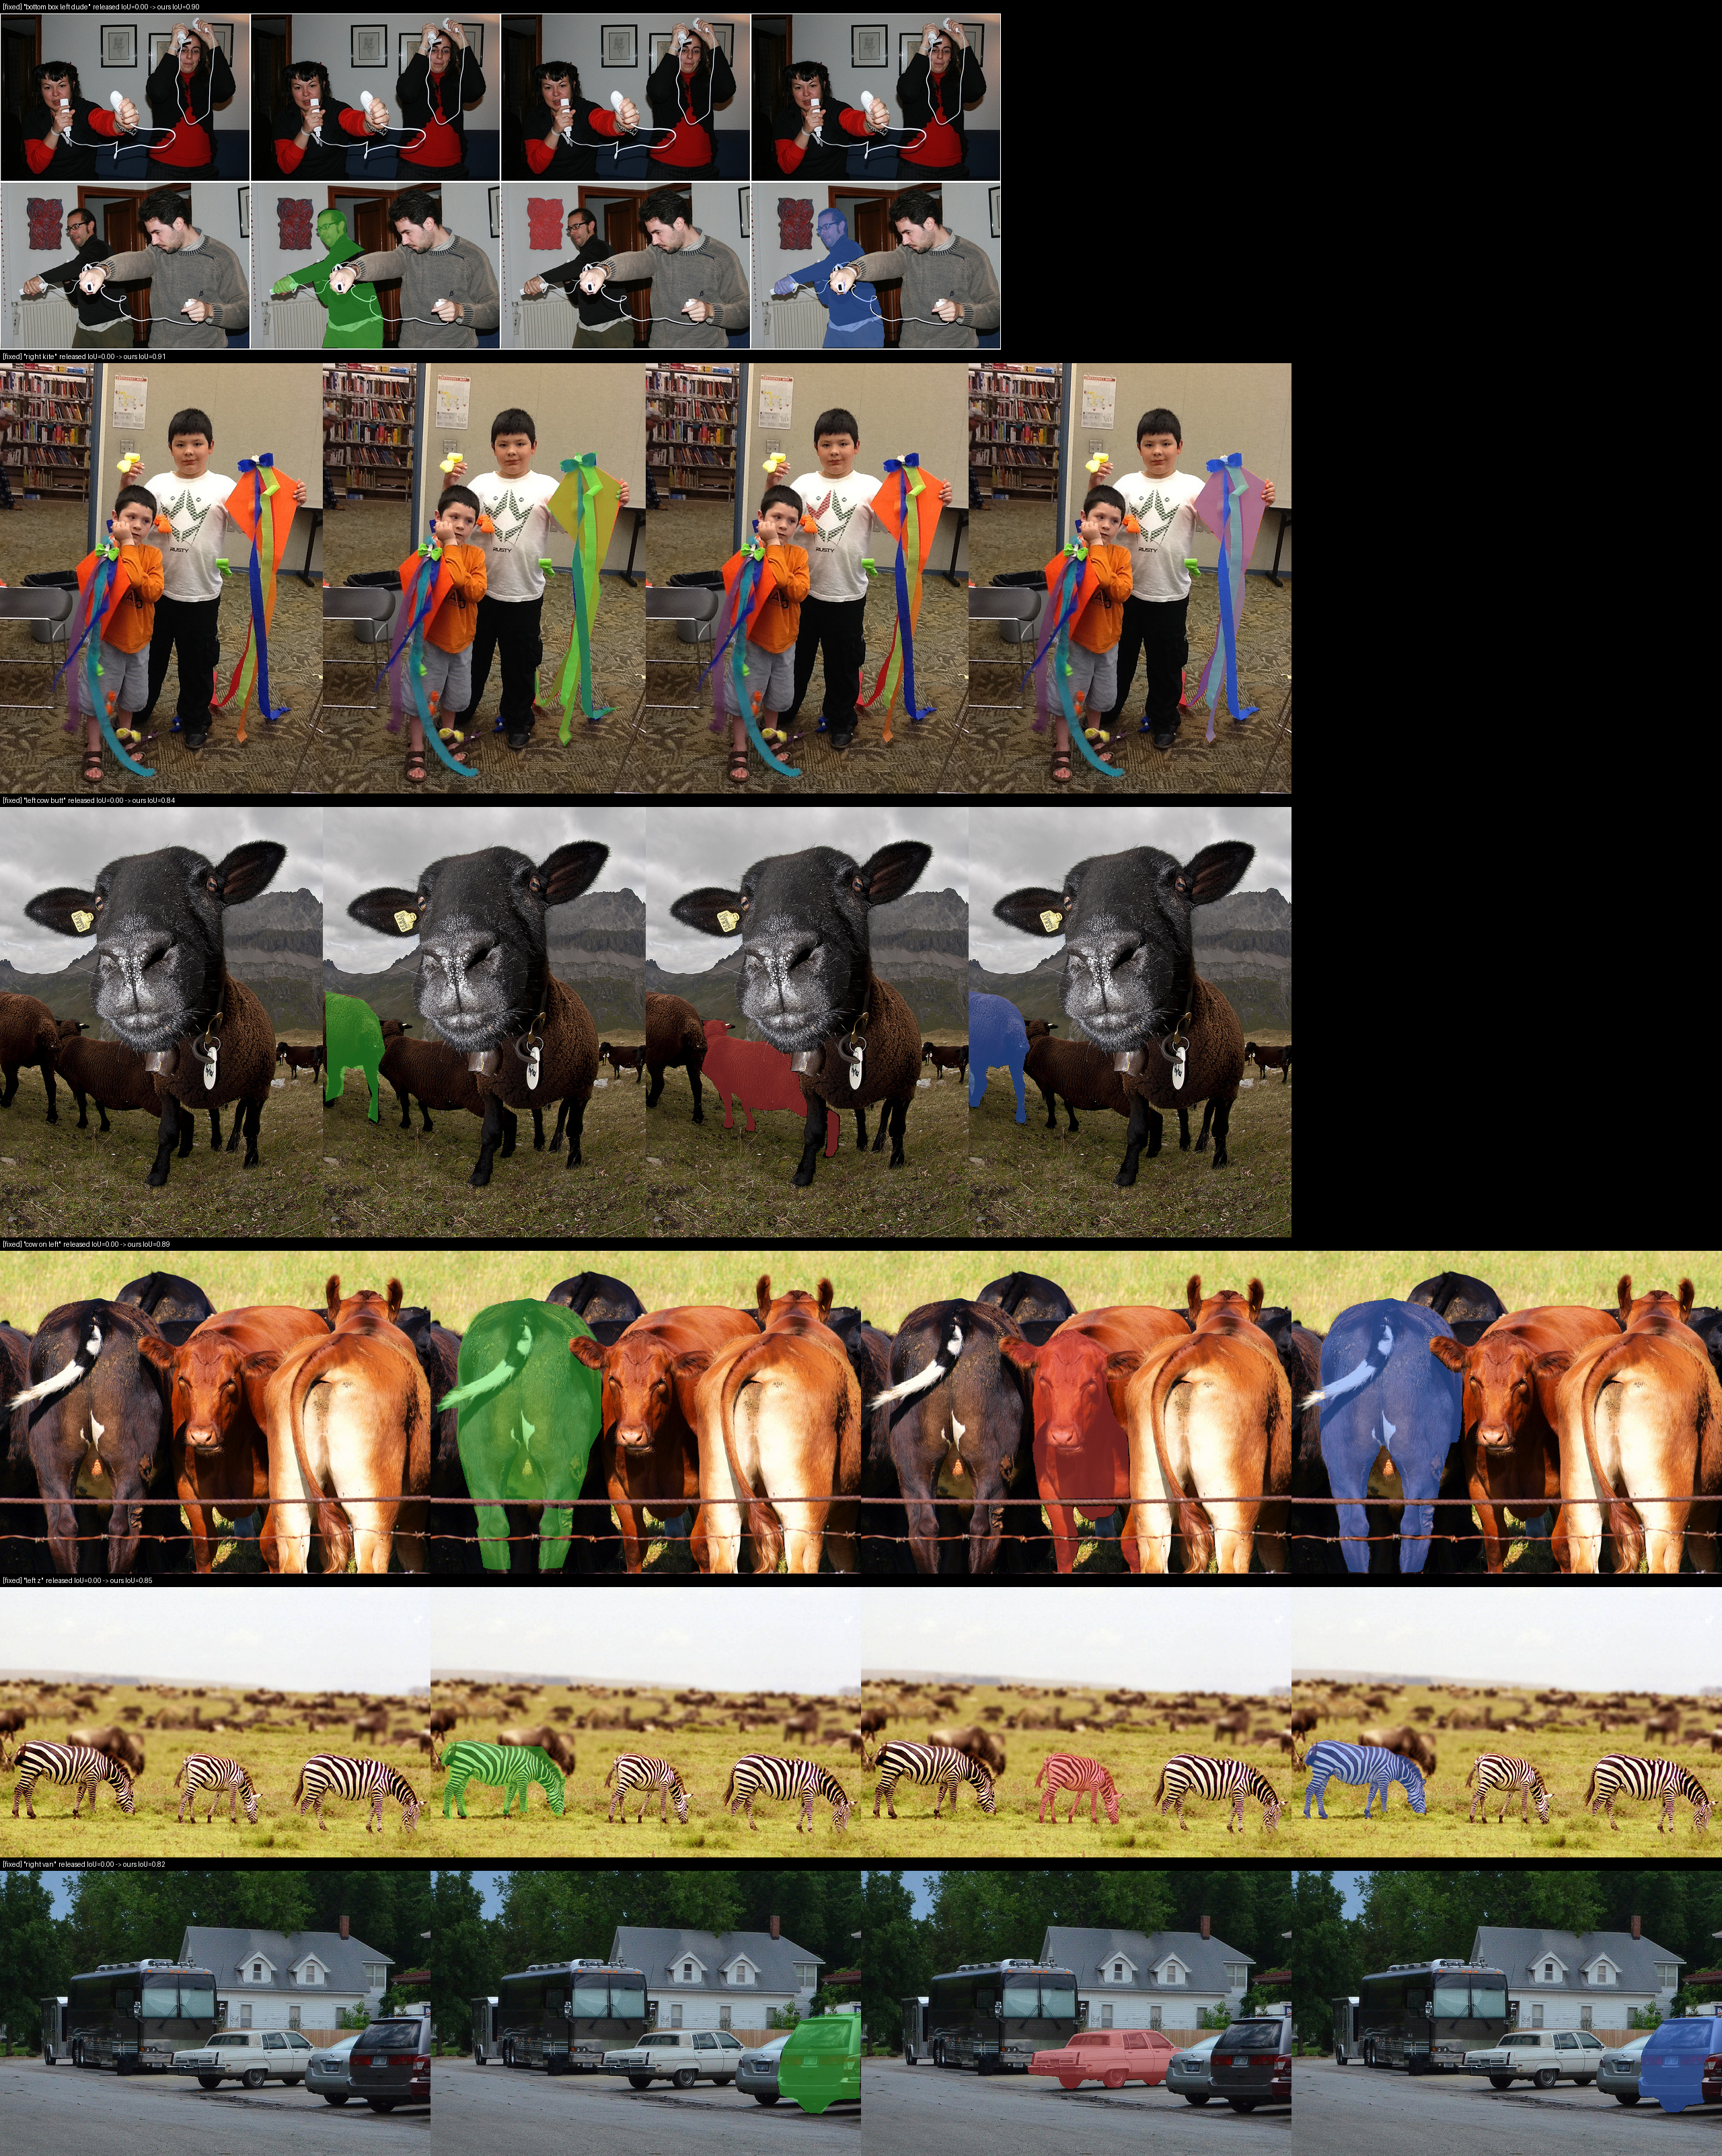
\includegraphics[width=\textwidth]{figures/qual_fixed.png}
\caption{Expressions the operator repairs. Columns: input; ground truth
(green); the released HybridGL selection (red); ours (blue). Rows are ordered by
reference id and are a deterministic sample, not a curated selection. In each
case the released pipeline returns a plausible instance of the right category
and the operator returns the referred one.}
\label{fig:qual}
\end{figure*}

Fig.~\ref{fig:qual} shows expressions on which the operator changes the
answer. The pattern is uniform and matches the diagnosis: the released pipeline
selects a real object of the correct category --- another person, another
sheep, another horse, another car --- and the operator selects the referred one.
This is the failure mode that dominates the oracle gap table, made visible.
